


\tikzset{every picture/.style={line width=0.75pt}} %set default line width to 0.75pt        

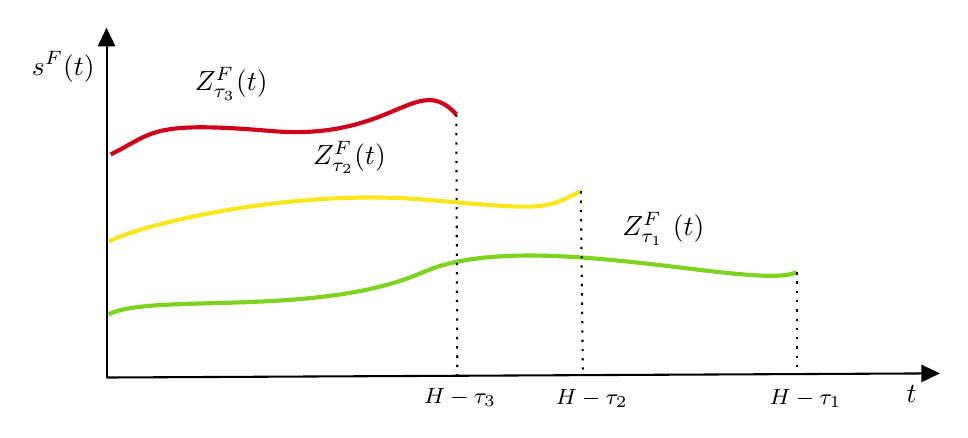
\begin{tikzpicture}[x=0.75pt,y=0.75pt,yscale=-1,xscale=1]
	%uncomment if require: \path (0,300); %set diagram left start at 0, and has height of 300
	
	%Curve Lines [id:da3576386679434109] 
	\draw [color={rgb, 255:red, 126; green, 211; blue, 33 }  ,draw opacity=1 ][line width=1.5]    (41.5,149.75) .. controls (62.66,139.39) and (143,151.5) .. (193,129.5) .. controls (243,107.5) and (354.16,138.73) .. (373,129.5) ;
	%Straight Lines [id:da044701537193025276] 
	\draw [line width=0.75]    (40.5,180.25) -- (439,178.26) ;
	\draw [shift={(442,178.25)}, rotate = 179.71] [fill={rgb, 255:red, 0; green, 0; blue, 0 }  ][line width=0.08]  [draw opacity=0] (8.93,-4.29) -- (0,0) -- (8.93,4.29) -- cycle    ;
	%Straight Lines [id:da0008580645658053943] 
	\draw [line width=0.75]    (40.5,180.25) -- (40.5,14.75) ;
	\draw [shift={(40.5,11.75)}, rotate = 90] [fill={rgb, 255:red, 0; green, 0; blue, 0 }  ][line width=0.08]  [draw opacity=0] (8.93,-4.29) -- (0,0) -- (8.93,4.29) -- cycle    ;
	%Curve Lines [id:da6528039000875612] 
	\draw [color={rgb, 255:red, 248; green, 231; blue, 28 }  ,draw opacity=1 ][line width=1.5]    (41.5,114.75) .. controls (62.66,104.39) and (134,89.5) .. (193,94.5) .. controls (252,99.5) and (250.16,99.73) .. (269,90.5) ;
	%Curve Lines [id:da6773052220718958] 
	\draw [color={rgb, 255:red, 208; green, 2; blue, 27 }  ,draw opacity=1 ][line width=1.5]    (42.5,72.75) .. controls (63.66,62.39) and (61,56.5) .. (120,61.5) .. controls (179,66.5) and (190,32.5) .. (209,53.5) ;
	%Straight Lines [id:da36906188743755486] 
	\draw  [dash pattern={on 0.84pt off 2.51pt}]  (209,53.5) -- (209.5,179.75) ;
	%Straight Lines [id:da5037794242478335] 
	\draw  [dash pattern={on 0.84pt off 2.51pt}]  (269,90.5) -- (270,179.25) ;
	%Straight Lines [id:da2541577667107384] 
	\draw  [dash pattern={on 0.84pt off 2.51pt}]  (373,129.5) -- (373,179.25) ;
	
	% Text Node
	\draw (424.5,182.37) node [anchor=north west][inner sep=0.75pt]    {$t$};
	% Text Node
	\draw (3,21.8) node [anchor=north west][inner sep=0.75pt]    {$s^{F}( t)$};
	% Text Node
	\draw (81.5,29.24) node [anchor=north west][inner sep=0.75pt]    {$Z_{\tau _{3}}^{F}( t)$};
	% Text Node
	\draw (138.5,64.74) node [anchor=north west][inner sep=0.75pt]    {$Z_{\tau _{2}}^{F}( t)$};
	% Text Node
	\draw (287.5,99.24) node [anchor=north west][inner sep=0.75pt]    {$Z_{\tau _{1\ }}^{F}( t)$};
	% Text Node
	\draw (358.5,184.37) node [anchor=north west][inner sep=0.75pt]  [font=\footnotesize]  {$H-\tau _{1}$};
	% Text Node
	\draw (255.5,184.37) node [anchor=north west][inner sep=0.75pt]  [font=\footnotesize]  {$H-\tau _{2}$};
	% Text Node
	\draw (192,183.87) node [anchor=north west][inner sep=0.75pt]  [font=\footnotesize]  {$H-\tau _{3}$};
	
	
\end{tikzpicture}